%#########settings########
\setlength{\parindent}{2ex}
\phantomsection
%##########text###########
%--------------------Task[1]--------------------
\section{Model the application using 3 Sequence Diagrams}
The following actions in all 3 Sequence Diagrams presented bellow are \textbf{common for all users}:\par
\begin{enumerate}
\item[•] \textbf{AplicationStartup()} represents the initialization of the application and it returns the Interface output to all types of users through \textbf{OutputInterface()}
\item[•] \textbf{Continue(selection)} represents the passing point from initial login form to the selection form.It request the form from the database through \textbf{RequestContinue(selection)} and returns the form through \textbf{ReturnContinue()}
\item[•] \textbf{Continue(output)} represents the passing point from selection from to the output form.It request the form from the database through \textbf{RequestContinue(output)} and returns the form through \textbf{ReturnContinue()}
once done the output is show to the user by \textbf{OutputForm()}.
\item[•] \textbf{UpdateView()} from \textit{output form} represents a view update that will give the readable onscreen filtered data to the user by \textbf{OutputFilteredView()} it will request the \textbf{UpdateView()} from the database apply the filter previously set \textbf{"ApplyFilter()"} then a request of data from the TrackMethods will be done "\textbf{GetData()} and \textbf{GetDataReturn()}" then the data will be returned to the interface through \textbf{ReturnUpdateView()}
\item[•] \textbf{SaveData()} represents a similar execution of \textbf{UpdateView()} just that the output will be in a specific data format;It will request the \textbf{SaveData()} from the database apply the filter previously set \textbf{"ApplyFilter()"} then a request of data from the TrackMethods will be done "\textbf{GetData()} and \textbf{GetDataReturn()}" then the data will be returned to the interface through \textbf{SaveDataReturn()} and the user will get the save the data\textit{.format} through \textbf{SaveDataFormat()}  
\item[•] \textbf{OpenData()} is a instance that will be issued by the user to open a data.\textit{format} from his OS and use the \textbf{SetFilter()},\textbf{UpdateView()} and \textbf{SaveData()} with the context of the data that was opened with \textbf{OpenData()} request to the Local OS Database and returned with \textbf{OpenDataReturn()} and \textbf{OutputDataForm()}
\end{enumerate}
\newpage
\textbf{Sequence diagram} \textnumero{1}
\begin{itemize}
\item[•] \textbf{AllowOnline()} is a checkbox for \textbf{SetMode(pass,online)} but this option isn't needed nor can be checked for \textit{\textbf{OfflineUser}} therefor it is unchecked.
\item[•] \textbf{MethodsSelection()} represents the selection of tracking messages that is then transmitted to the database to ask for their initialization through \textbf{InitializationMethods()} and individual initialization through \textbf{StartMethods()}
\item[•] \textbf{SetFilter()} represents the setting of a filter the the data that will be saved in the database and then used in \textbf{UpdateView()},\textbf{OpenData()} and \textbf{SaveData()} through \textbf{ApplyFilter()}.
\end{itemize}
\newpage
\begin{figure}[!h]
	\centering
	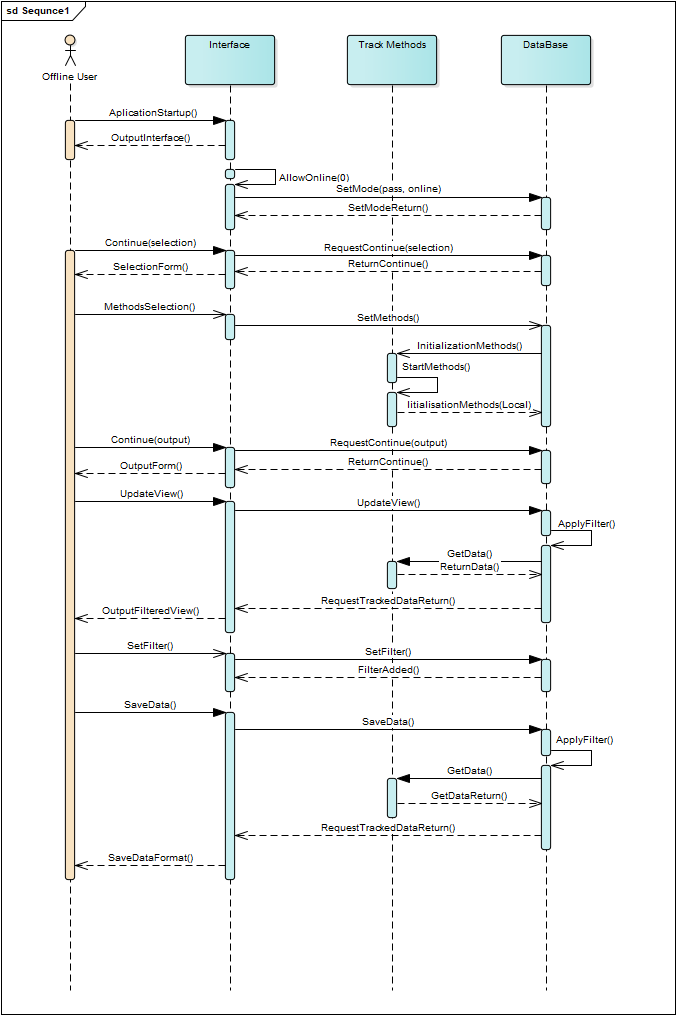
\includegraphics[keepaspectratio=true,scale=0.65]{Sequence1}
	\caption{OfflineUser} 
\end{figure}
%-------------[1]
\newpage 
\textbf{Sequence diagram} \textnumero{2}
\begin{itemize}
\item[•] \textbf{Addpass()} represents the input of a password in the initialization from where the user sets the mode he wants to work in; As the user is operating in \textbf{Online(Admin)}:
\begin{itemize}
\item \textbf{SetPass()} sets a security password in the database, which allows checking the \textbf{AllowOnline()} to be checked and afterwards saving the mode through \textbf{SetMode(pass,online)} in database which will allow to access \textbf{AddTrackID(ID,Pass)}.
\
\item \textbf{AddTrackID(ID,Pass)} represents an option to add as many ID's with their respective password to track.
\end{itemize}
\item[•] \textbf{MethodsSelection()} represents the selection of tracking messages that is then transmitted to the database to ask for their initialization through \textbf{InitializationMethods()} and individual initialization through \textbf{StartMethods()} and will return the activation response through \textbf{InitializationMethods(Local)} afterwards it will send and request to the local users that the admin has choosed to track \textbf{AdminMethods(Send)} and will receive through \textbf{AdminMethods(return)} if the user is connected and will see the output on screen through \textbf{LocalUserConnected():Yes}.
\item[•] \textbf{SetFilter()} represents the setting of a filter the the data that will be saved in the database thorough \textbf{SetFilter()} function which will afterwards send the filter to the local users and request the filtered data \textbf{RequestData()},\textbf{ReturnRequestData()} and then used in \textbf{UpdateView()},\textbf{OpenData()} and \textbf{SaveData()} through \textbf{ApplyFilter()}.
\end{itemize}
\newpage
\begin{figure}[!h]
	\centering
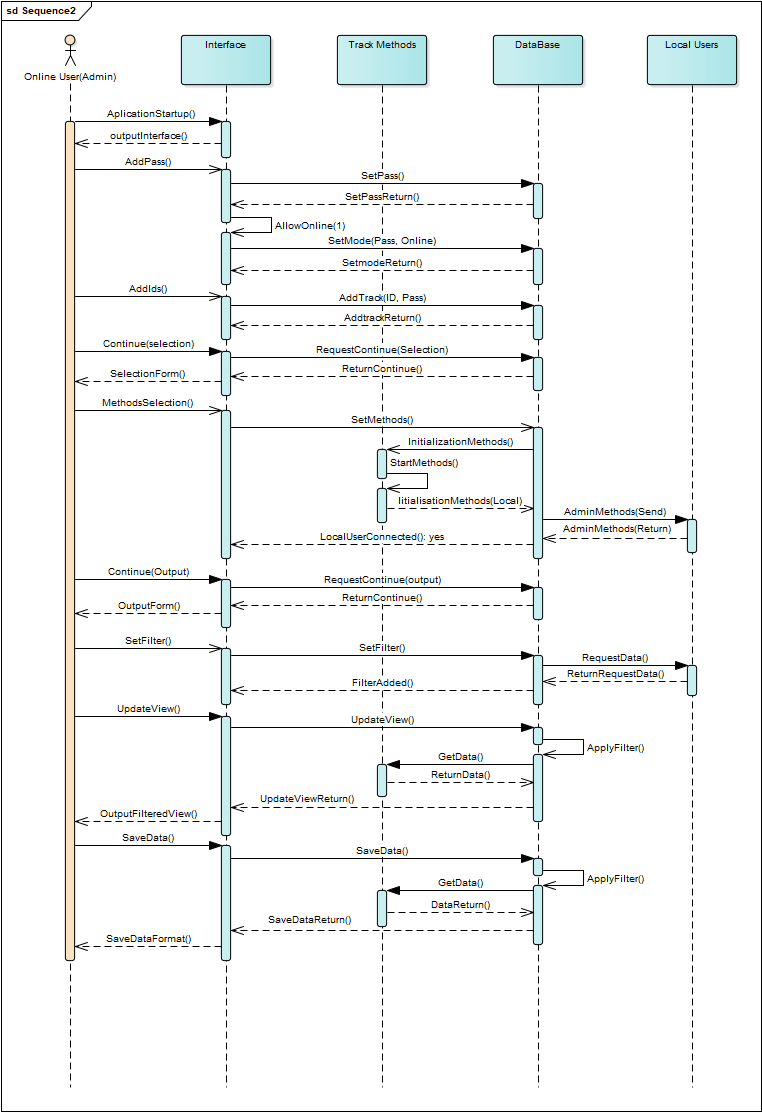
\includegraphics[keepaspectratio=true,scale=0.6]{Sequence2}
	\caption{OnlineUser(Admin)} 
\end{figure}
%-------------[2]
\newpage
\textbf{Sequence diagram} \textnumero{3}
\begin{itemize}
\item[•] \textbf{SetPass()} sets a security password in the database, which allows checking the \textbf{AllowOnline()} to be checked and afterwards saving the mode through \textbf{SetMode(pass,online)} in database.
\item[•] \textbf{MethodsSelection()} represents the selection of tracking messages that is then transmitted to the database to ask for their initialization through \textbf{InitializationMethods()} and individual initialization through \textbf{StartMethods()} and will return the activation response through \textbf{InitializationMethods(Local)} afterwards 
if it will receive the \textbf{AdminMethods(send)} from the admin of the group which will ask for initialization of the methods that weren't initialized through \textbf{InitializationMethods()} and individual initialization through \textbf{StartMethods()} and will return the activation response through \textbf{InitializationMethods(Admin)}
\item[•] \textbf{SetFilter()} represents the setting of a filter the the data that will be saved in the database thorough \textbf{SetFilter()} function which will be used in \textbf{UpdateView()},\textbf{OpenData()} and \textbf{SaveData()} through \textbf{ApplyFilter()}.
\end{itemize}
\newpage
\begin{figure}[!h]
	\centering
	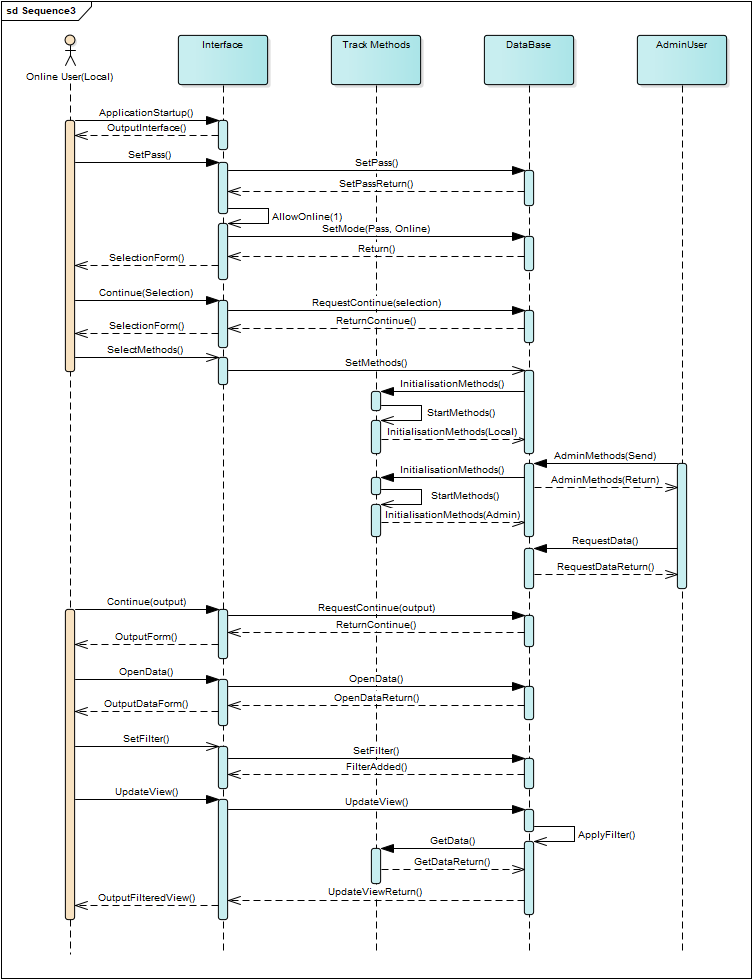
\includegraphics[keepaspectratio=true,scale=0.65]{Sequence3}
	\caption{OnlineUser(Local)} 
\end{figure}
%-------------[3]
%--------------------Task[2]--------------------
\newpage
\section{Analyze the Functional and Non-Functional Requirements for the project.}
\textbf{Functional Requirements}
\begin{enumerate}
\item[•] For Track Methods to save tracked data in statistic form.
\item[•] For Track Methods to ask for the permissions from the user of what data can be tracked.
\item[•] For Filter to show what data can be accessed and requested from the database.
\item[•] For Showing the user how to use the Output form.
\end{enumerate}
\textbf{Non-Functional Requirements}
\begin{enumerate}
\item[•] Product Requirements:
\begin{itemize}
\item Number of Processor: 2
\item Disk capacity min: 6Gb
\item Operating system: Windows ,Ubuntu,Mac Os
\item Database vendor: Microsoft(MySql)
\end{itemize}
\item[•] Efficiency requirements:\par
The application should operate with local users tracked data connected with an admin in within a reasonable time.
\item[•] Portability requirements:\par 
The application should run all modern operating systems and be able to interface major relational database systems from various vendors.
\item[•] Privacy requirements:\par The application should not reveal private passwords nor any tracked data to outside of network local/admin users.
\end{enumerate}
\clearpage
